\documentclass[10pt, a4paper, onecolumn, oneside, titlepage, openany]{book}

\usepackage[T1]{fontenc}    %% TeX text extended - most European characters
\usepackage[utf8]{inputenc} %% UTF-8 support
\usepackage{menukeys}       %% keyboads keys, menu + includes '\definecolor'

\usepackage{hyperref}       %% URL and reference support
\hypersetup{
    colorlinks=true,
    linkcolor=blue,         %% \ref{}
    filecolor=magenta,      %% \href{run:./file.txt}{File.txt}
    urlcolor=cyan,          %% \href{http://www.overleaf.com}{Link}
    pdfpagemode=FullScreen,
    pdftitle={Linux Artix}
}

\usepackage{titlesec}       %% chapter formatting (N. CHAPTER-NAME)
\renewcommand{\chaptername}{}
\titleformat{\chapter}[hang]{\normalfont\huge\bfseries}{\chaptertitlename\ \thechapter.}{1em}{}

\usepackage{fancyhdr}       %% decorative lines
\renewcommand{\headrulewidth}{2pt}
\renewcommand{\footrulewidth}{2pt}
\pagestyle{fancy}
\fancyhf{}
    \chead{\leftmark}
    \cfoot{\thepage}
\fancypagestyle{plain}{
\fancyhf{}
    \chead{\leftmark}
    \cfoot{\thepage}
}

%% table formatting
\usepackage[format=hang,font=small,labelfont=bf]{caption} %% bold table caption
\setlength{\arrayrulewidth}{0.5mm}                        %% border
\setlength{\tabcolsep}{18pt}                              %% space from border (X axis)
\renewcommand{\arraystretch}{1.5}                         %% space from border (Y axis)

%% colors
\definecolor{bg}{RGB}{240, 240, 240}
\definecolor{root}{RGB}{222, 0, 0}
\definecolor{user}{RGB}{0, 150, 0}
\definecolor{command}{RGB}{41, 182, 0}
\definecolor{block}{RGB}{255, 80, 0}
\definecolor{dir}{RGB}{0, 100, 200}
\definecolor{file}{RGB}{77, 187, 101}
\definecolor{comment}{RGB}{0, 182, 182}

%% code formatting
\usepackage{fancyvrb}
\renewcommand{\FancyVerbFormatLine}[1]{\colorbox{bg}{#1}}




\title{\textbf{Linux Artix}}
\author{AISK11}
\date{March 2022}

\begin{document}
\maketitle
\tableofcontents


\chapter{System Info}
%\section{System Hardware}
\begin{table}[!ht]
\centering
\begin{tabular}{|c|c|}
    \hline
    \textbf{Hardware} & \textbf{Value} \\
    \hline
    CPU architecture & amd64\\
    CPU vendor & intel\\
    Motherboard & UEFI\\
    Hard Drive & NVMe\\
    WiFi & iwlwifi\\
    GPU & Intel + Nvidia\\
    \hline
\end{tabular}
\caption{System hardware overview.}
\label{table:1}
\end{table}

%\section{System Software}
\begin{table}[!ht]
\centering
\begin{tabular}{|c|c|}
    \hline
    \textbf{Software} & \textbf{Value} \\
    \hline
    RAID & -\\
    LVM & -\\
    Encryption & LUKS\\
    Root filesystem & btrfs\\
    SWAP & 4GB (file)\\
    Bootloader & rEFInd\\
    Kernel & linux (artix)\\
    Initramfs & dracut\\
    Init & dinit\\
    Shell & zsh\\
    Virtualization & ?\\
    \hline
\end{tabular}
\caption{System software overview.}
\label{table:2}
\end{table}

%\section{Display Software}
\begin{table}[!ht]
\centering
\begin{tabular}{|c|c|}
    \hline
    \textbf{Software} & \textbf{Value} \\
    \hline
    Display server & Xorg\\
    Window manager & bspwm\\
    Desktop environment & -\\
    Terminal emulator & rxvt-unicode\\
    \hline
\end{tabular}
\caption{Display software overview.}
\label{table:3}
\end{table}


\chapter{Download and Boot}
\section{Download Artix ISO}
\begin{enumerate}
    \item \textbf{Download Artix ISO}
    \begin{itemize}
        \item \textbf{Artix download page:}
\newline \url{https://artixlinux.org/download.php}
        \item \textbf{Select install file:}
\newline \menu[,]{Official ISO images, base, artix-base-dinit-<YYYYMMDD>-x86\_64.iso}
    \end{itemize}
    \item \textbf{Verify download: @TODO}
\end{enumerate}

\section{USB Preparation}
\begin{enumerate}
    \item \textbf{Unmount USB FS!}
    \item \textbf{Flash image to USB:}
\begin{Verbatim}[commandchars=\\\{\}]
\textcolor{root}{root#} \textcolor{command}{dd} if=<\textcolor{file}{./artix-base-runit-<YYYYMMDD>-x86_64.iso>.iso}> of=<\textcolor{block}{/dev/sdX}>
[bs=4M] [conv=fsync] [status=progress] && \textcolor{command}{sync}
\end{Verbatim}
\end{enumerate}

\section{Boot USB}
\subsection{Disable Secure Boot}
\begin{enumerate}
    \item \textbf{During POST press key to access BIOS/UEFI:}
\newline \href{https://techofide.com/blogs/boot-menu-option-keys-for-all-computers-and-laptops-updated-list-2021-techofide/}{https://techofide.com/blogs/boot-menu-option-keys-for-all-computers-and-laptops-updated-list-2021-techofide/}
    \item \textbf{Disable Secure Boot.}
    \item \textbf{Poweroff/Restart.}
\end{enumerate}
\subsection{Boot}
\begin{enumerate}
    \item \textbf{Plug in flashed USB.}
    \item \textbf{During POST press key to access Boot Menu:}
\newline \href{https://techofide.com/blogs/boot-menu-option-keys-for-all-computers-and-laptops-updated-list-2021-techofide/}{https://techofide.com/blogs/boot-menu-option-keys-for-all-computers-and-laptops-updated-list-2021-techofide/}
    \item \textbf{Select USB entry (UEFI).}
\end{enumerate}


\chapter{Pre-Installation}
\section{Login}
\begin{itemize}
    \item \textbf{Login to live environment:}
\begin{Verbatim}[commandchars=\\\{\}]
> artix
> artix
\end{Verbatim}
    \item \textbf{Access root:}
\begin{Verbatim}[commandchars=\\\{\}]
\textcolor{user}{user\$} \textcolor{command}{sudo} passwd root
> <NEW_ROOT_PASSWORD>
> <NEW_ROOT_PASSWORD (VERIFY)>
\textcolor{user}{user\$} \textcolor{command}{su} -
\end{Verbatim}
\end{itemize}

\section{Disable pcspkr Module}
\begin{enumerate}
    \item \textbf{See if pcspkr is active:}  
\begin{Verbatim}[commandchars=\\\{\}]
\textcolor{root}{root#} \textcolor{command}{lsmod} | \textcolor{command}{grep} -i pcspkr
\end{Verbatim}
    \item \textbf{Disable pcspkr module:}
\begin{Verbatim}[commandchars=\\\{\}]
\textcolor{root}{root#} \textcolor{command}{modprobe} -r pcspkr
\end{Verbatim}
\end{enumerate}

\section{Verify UEFI}
\begin{itemize}
    \item \textbf{UEFI is used if following directory exists:}
\newline \textbf{\textcolor{dir}{/sys/firmware/efi/}}
    \item \textbf{Verify via kernel:}
\begin{Verbatim}[commandchars=\\\{\}]
\textcolor{root}{root#} \textcolor{command}{dmesg} | \textcolor{command}{grep} -i efi
\end{Verbatim}
\end{itemize}

\section{Connect To The Internet}
\begin{enumerate}
    \item \textbf{Connect to the internet:}
\newline See section: \underline{\textbf{\ref{network}}}.
\end{enumerate}

\section{Time Sync}
\begin{enumerate}
    \item \textbf{Synchronize time:}
\newline See section: \underline{\textbf{\ref{datetime}}}.
\end{enumerate}

\section{Install Additional Software}
\begin{enumerate}
    \item \textbf{Synchronize database:}
\begin{Verbatim}[commandchars=\\\{\}]
\textcolor{root}{root#} [\textcolor{command}{yes} |] \textcolor{command}{pacman} -Syy
\end{Verbatim}
    \item \textbf{Install parted:}
\begin{Verbatim}[commandchars=\\\{\}]
\textcolor{root}{root#} [\textcolor{command}{yes} |] \textcolor{command}{pacman} -S [--needed] parted
\end{Verbatim}
\end{enumerate}

\section{Check Disk Sectors}
\subsection{Theory}
\begin{itemize}
    \item \textbf{Sector:} smallest unit size on disk. 512 or 4096 bytes (Advanced Format). 4096 Advanced Format disks have usually 512-byte conversion firmware.
    \item \textbf{Block:} allocation size the FS uses. Cannot be smaller than size of the sector. Can be group of sectors (4096b: 8 x 512b sectors).
    \begin{itemize}
        \item \textbf{512b =} good for lot of small files. More blocks = more metadata.
        \item \textbf{4096b =}  good for larger files, less metadata. Waste if there are mostly small files.
    \end{itemize}
\end{itemize}
\subsection{Disk Information}
\begin{itemize}
    \item \textbf{Find disks (block devices):}
\begin{Verbatim}[commandchars=\\\{\}]
\textcolor{user}{user\$} \textcolor{command}{lsblk} [-ap | -apf]
\textcolor{root}{root#} \textcolor{command}{fdisk -l} [\textcolor{block}{/dev/sdX}]
\textcolor{root}{root#} \textcolor{command}{gdisk -l} <\textcolor{block}{/dev/sdX}>
\textcolor{root}{root#} \textcolor{command}{blkid}
\end{Verbatim}
    \item \textbf{Get raw disk info:}
    \begin{itemize}
        \item \textbf{Get disk physical sector size:}
\begin{Verbatim}[commandchars=\\\{\}]
\textcolor{root}{root#} \textcolor{command}{blockdev} [-v] --getpbsz <\textcolor{block}{/dev/sdX[Y]}>
\end{Verbatim}
        \item \textbf{Get disk logical sector size (usually 512):}
\begin{Verbatim}[commandchars=\\\{\}]
\textcolor{root}{root#} \textcolor{command}{blockdev} [-v] --getss <\textcolor{block}{/dev/sdX[Y]}>
\end{Verbatim}
        \item \textbf{Disk size in bytes:}
\begin{Verbatim}[commandchars=\\\{\}]
\textcolor{root}{root#} \textcolor{command}{blockdev} [-v] --getsize64 <\textcolor{block}{/dev/sdX[Y]}>
\end{Verbatim}
    \item \textbf{Check if disk is readonly (1 = ro, 0 = rw):}
\begin{Verbatim}[commandchars=\\\{\}]
\textcolor{root}{root#} \textcolor{command}{blockdev} [-v] --getro <\textcolor{block}{/dev/sdX[Y]}>
\end{Verbatim}
    \end{itemize}
    \item \textbf{See partitions:}
\begin{Verbatim}[commandchars=\\\{\}]
\textcolor{root}{root#} \textcolor{command}{parted} -s <\textcolor{block}{/dev/sdX}> (p)rint [free]
\end{Verbatim}
\end{itemize}
\subsection{Check Disk For Bad Sectors}
\begin{enumerate}
    \item \textbf{Unmount FS!}
    \item \textbf{Check disk for bad blocks:}
\begin{Verbatim}[commandchars=\\\{\}]
\textcolor{root}{root#} \textcolor{command}{badblocks} [-b 4096] [-w [-t 0xaa]] [-v] [-s]
<\textcolor{block}{/dev/sdX[Y]}> | \textcolor{command}{tee} -a <\textcolor{file}{OUTPUT_FILE}>
\end{Verbatim}
\end{enumerate}


\chapter{Installation}
\section{Disk Partitioning}
\begin{figure}[ht]
    \begin{center}
        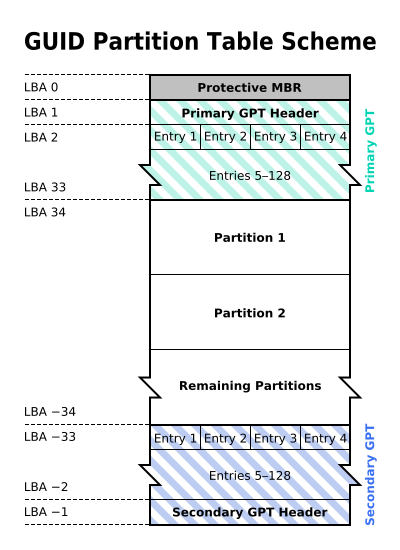
\includegraphics[width=40mm]{./src/img/gpt1.png}
        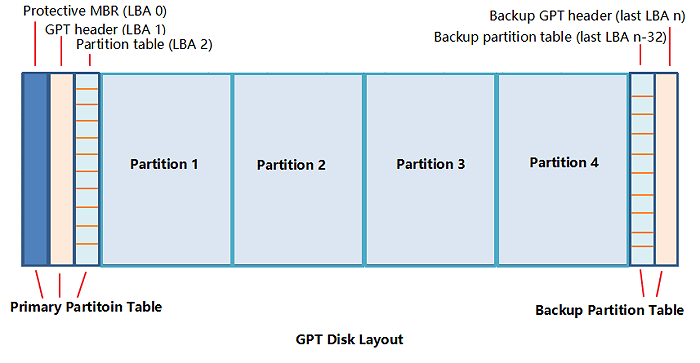
\includegraphics[width=75mm]{./src/img/gpt2.png}
        \caption{GPT Partition Table.}
        \label{fig:1}
    \end{center}
\end{figure}
\subsection{Partition Table}
\begin{enumerate}
    \item \textbf{Unmount FS from disk on which linux will be installed!}
    \item \textbf{Create GPT partition table:}
\begin{Verbatim}[commandchars=\\\{\}]
\textcolor{root}{root#} \textcolor{command}{parted} -s <\textcolor{block}{/dev/sdX}> mktable gpt
\end{Verbatim}
\end{enumerate}
\subsection{Basic Partitions}
\begin{enumerate}
    \item \textbf{Enter cfdisk:}
\begin{Verbatim}[commandchars=\\\{\}]
\textcolor{root}{root#} \textcolor{command}{cfdisk} <\textcolor{block}{/dev/sdX}>
\end{Verbatim}
    \item \textbf{Create EFI partition (recommended 550 MiB):}
\begin{Verbatim}[commandchars=\\\{\}]
\textcolor{root}{cfdisk>} \textcolor{command}{n}
\textcolor{root}{cfdisk>} \textcolor{command}{550MiB}
\textcolor{root}{cfdisk>} \textcolor{command}{t}
\textcolor{root}{cfdisk>} \textcolor{command}{EFI System}
\end{Verbatim}
    \item \textbf{Create encrypted partition:}
\begin{Verbatim}[commandchars=\\\{\}]
\textcolor{root}{cfdisk>} \textcolor{command}{n}
\textcolor{root}{cfdisk>} \textcolor{command}{} (Enter)
\end{Verbatim}
    \item \textbf{Write changes:}
\begin{Verbatim}[commandchars=\\\{\}]
\textcolor{root}{cfdisk>} \textcolor{command}{W}
\textcolor{root}{cfdisk>} \textcolor{command}{yes}
\end{Verbatim}
    \item \textbf{Quit cfdisk:}
\begin{Verbatim}[commandchars=\\\{\}]
\textcolor{root}{cfdisk>} \textcolor{command}{Q}
\end{Verbatim}
    \item \textbf{Name partitions:}
\begin{Verbatim}[commandchars=\\\{\}]
\textcolor{root}{root#} \textcolor{command}{parted} -s <\textcolor{block}{/dev/sdX}> name 1 ESP
\textcolor{root}{root#} \textcolor{command}{parted} -s <\textcolor{block}{/dev/sdX}> name 2 LUKS
\end{Verbatim}
    \item \textbf{Format partitions:}
    \begin{enumerate}
        \item \textbf{ESP:}
\begin{Verbatim}[commandchars=\\\{\}]
\textcolor{root}{root#} \textcolor{command}{mkfs.fat} -F 32 <\textcolor{block}{/dev/sdX1}>
\textcolor{root}{root#} \textcolor{command}{fatlabel} <\textcolor{block}{/dev/sdX1}> <ESP>
\end{Verbatim}
        \item \textbf{LUKS:}
\begin{Verbatim}[commandchars=\\\{\}]
\textcolor{root}{root#} \textcolor{command}{cryptsetup} luksFormat --label <LUKS> <\textcolor{block}{/dev/sdX2}>
> YES
> <NEW_LUKS_PASSWORD>
> <NEW_LUKS_PASSWORD (VERIFY)>
\end{Verbatim}
    \end{enumerate}
\end{enumerate}
    \subsection{(Advanced LUKS Stuff)}
\begin{itemize}
    \item \textbf{Open LUKS:}
\begin{Verbatim}[commandchars=\\\{\}]
\textcolor{root}{root#} \textcolor{command}{cryptsetup} open --type luks <\textcolor{block}{/dev/sdX2}> <luks>
> <PASSWORD>
\end{Verbatim}
    \item \textbf{Close LUKS:}
\begin{Verbatim}[commandchars=\\\{\}]
\textcolor{root}{root#} \textcolor{command}{cryptsetup} close <luks>
\end{Verbatim}
    \item \textbf{LUKS header:}
    \begin{enumerate}
        \item \textbf{See LUKS header:}
\begin{Verbatim}[commandchars=\\\{\}]
\textcolor{root}{root#} \textcolor{command}{cryptsetup} luksDump <\textcolor{block}{/dev/sdX2}>
\end{Verbatim}
        \item \textbf{Make LUKS header backup:}
\begin{Verbatim}[commandchars=\\\{\}]
\textcolor{root}{root#} \textcolor{command}{cryptsetup} luksHeaderBackup <\textcolor{block}{/dev/sdX2}>
--header-backup-file <\textcolor{file}{FILE}>
\end{Verbatim}
        \item \textbf{Destroy LUKS header:}
\begin{Verbatim}[commandchars=\\\{\}]
\textcolor{root}{root#} \textcolor{command}{cryptsetup} luksErase <\textcolor{block}{/dev/sdX2}>
> YES
\end{Verbatim}
        \item \textbf{Restore LUKS header:}
\begin{Verbatim}[commandchars=\\\{\}]
\textcolor{root}{root#} \textcolor{command}{cryptsetup} luksHeaderRestore <\textcolor{block}{/dev/sdX2}>
--header-backup-file <\textcolor{file}{FILE}>
> YES
\end{Verbatim}
    \end{enumerate}
    \item \textbf{Passwords}
    \begin{itemize}
        \item \textbf{Change password:}
\begin{Verbatim}[commandchars=\\\{\}]
\textcolor{root}{root#} \textcolor{command}{cryptsetup} luksChangeKey <\textcolor{block}{/dev/sdX2}>
> <OLD_PASSWORD>
> <NEW_PASSWORD>
> <NEW_PASSWORD (VERIFY)>
\end{Verbatim}
    \end{itemize}
\end{itemize}
\subsection{Encrypted Partition}
\begin{figure}[ht]
    \begin{center}
        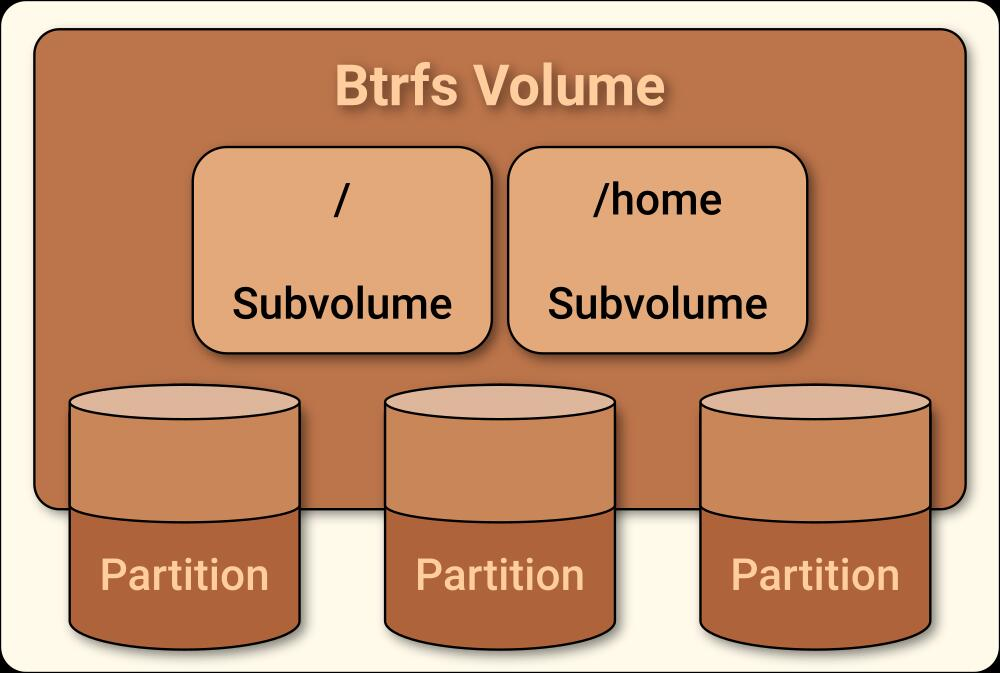
\includegraphics[width=75mm]{./src/img/btrfs.png}
        \caption{Btrfs structure.}
        \label{fig:2}
    \end{center}
\end{figure}
\begin{enumerate}
    \item \textbf{Open encrypted partition:}
\begin{Verbatim}[commandchars=\\\{\}]
\textcolor{root}{root#} \textcolor{command}{cryptsetup} open --type luks <\textcolor{block}{/dev/sdX2}> <luks-root>
> <PASSWORD>
\end{Verbatim}
    \item \textbf{Format root partition:}
\begin{Verbatim}[commandchars=\\\{\}]
\textcolor{root}{root#} \textcolor{command}{mkfs.btrfs} <\textcolor{block}{/dev/mapper/luks-root}>
\textcolor{root}{root#} \textcolor{command}{btrfs} filesystem label <\textcolor{block}{/dev/mapper/luks-root}> <LUKS-ROOT>
\end{Verbatim}
\end{enumerate}

\section{Base Artix Installation}
\begin{enumerate}
    \item \textbf{Create mount directory:}
\begin{Verbatim}[commandchars=\\\{\}]
\textcolor{root}{root#} \textcolor{command}{mkdir} <\textcolor{dir}{/mnt/artix/}>
\end{Verbatim}
    \item \textbf{Mount Artix:}
\begin{Verbatim}[commandchars=\\\{\}]
\textcolor{root}{root#} \textcolor{command}{mount} <\textcolor{block}{/dev/mapper/luks-root}> <\textcolor{dir}{/mnt/artix/}>
\end{Verbatim}
    \item \textbf{Install packages to new directory:}
\begin{Verbatim}[commandchars=\\\{\}]
\textcolor{root}{root#} \textcolor{command}{basestrap} <\textcolor{dir}{/mnt/artix/}> base
\end{Verbatim}
\end{enumerate}

\section{Chroot}
\begin{enumerate}
    \item \textbf{Mount all filesystems:}
\begin{Verbatim}[commandchars=\\\{\}]
\textcolor{root}{root#} \textcolor{command}{mount} -t proc \textcolor{dir}{/proc/} <\textcolor{dir}{/mnt/artix/proc/}>
\textcolor{root}{root#} \textcolor{command}{mount} --rbind \textcolor{dir}{/sys/} <\textcolor{dir}{/mnt/artix/sys/}>
\textcolor{root}{root#} \textcolor{command}{mount} --make-rslave <\textcolor{dir}{/mnt/artix/sys/}>
\textcolor{root}{root#} \textcolor{command}{mount} --rbind \textcolor{dir}{/dev/} <\textcolor{dir}{/mnt/artix/dev/}>
\textcolor{root}{root#} \textcolor{command}{mount} --make-rslave <\textcolor{dir}{/mnt/artix/dev/}>
\textcolor{root}{root#} \textcolor{command}{mount} --bind \textcolor{dir}{/run/} <\textcolor{dir}{/mnt/artix/run/}>
\textcolor{root}{root#} \textcolor{command}{mount} --make-slave <\textcolor{dir}{/mnt/artix/run/}>
\end{Verbatim}
    \item \textbf{Chroot:}
\begin{Verbatim}[commandchars=\\\{\}]
\textcolor{root}{root#} \textcolor{command}{chroot} <\textcolor{dir}{/mnt/artix/}> \textcolor{file}{/bin/bash}
\textcolor{root}{root#} \textcolor{command}{source} \textcolor{file}{/etc/profile}
\textcolor{root}{root#} \textcolor{command}{export} PS1="(chroot) \$\{PS1\}"
\end{Verbatim}
    \item \textbf{Mount boot partition:}
\begin{Verbatim}[commandchars=\\\{\}]
\textcolor{root}{(chroot) root#} \textcolor{command}{mount} <\textcolor{block}{/dev/sdX1}> \textcolor{dir}{/boot/}
\end{Verbatim}
    \item \textbf{Add DNS server:}
\begin{Verbatim}[commandchars=\\\{\}]
\textcolor{root}{(chroot) root#} \textcolor{command}{echo} "nameserver 1.1.1.1" > \textcolor{file}{/etc/resolv.conf}
\end{Verbatim}
\end{enumerate}

\section{Pacman Configuration}
\begin{enumerate}
    \item \textbf{Add additional Arch packages:}
\begin{Verbatim}[commandchars=\\\{\}]
\textcolor{root}{(chroot) root#} [\textcolor{command}{yes} |] \textcolor{command}{pacman} -S [--needed] artix-archlinux-support
\end{Verbatim}
    \item \textbf{Pacman configuration:}
\newline File (\textbf{\textcolor{file}{/etc/pacman.conf}}):
\newline \url{https://github.com/AISK11/Artix/blob/main/configs/artix/pacman.conf}
    \item \textbf{Synchronize new repos [and update]:}
\begin{Verbatim}[commandchars=\\\{\}]
\textcolor{root}{(chroot) root#} [\textcolor{command}{yes} |] \textcolor{command}{pacman} -Syy[u]
\end{Verbatim}
\end{enumerate}

\section{Additional Packages}
\begin{itemize}
    \item \textbf{Text editor:}
\begin{Verbatim}[commandchars=\\\{\}]
\textcolor{root}{(chroot) root#} [\textcolor{command}{yes} |] \textcolor{command}{pacman} -S [--needed] vim
\end{Verbatim}
    \item \textbf{Git:}
\begin{Verbatim}[commandchars=\\\{\}]
\textcolor{root}{(chroot) root#} [\textcolor{command}{yes} |] \textcolor{command}{pacman} -S [--needed] git
\end{Verbatim}
    \item \textbf{Partitioning}
\begin{Verbatim}[commandchars=\\\{\}]
\textcolor{root}{(chroot) root#} [\textcolor{command}{yes} |] \textcolor{command}{pacman} -S [--needed] parted
\end{Verbatim}
    \item \textbf{Filesystems:}
\begin{Verbatim}[commandchars=\\\{\}]
\textcolor{root}{(chroot) root#} [\textcolor{command}{yes} |] \textcolor{command}{pacman} -S [--needed] dosfstools cryptsetup 
btrfs-progs
\end{Verbatim}
    \item \textbf{Bootloader:}
\begin{Verbatim}[commandchars=\\\{\}]
\textcolor{root}{(chroot) root#} [\textcolor{command}{yes} |] \textcolor{command}{pacman} -S [--needed] refind
\end{Verbatim}
     \item \textbf{Initramfs:}
\begin{Verbatim}[commandchars=\\\{\}]
\textcolor{root}{(chroot) root#} [\textcolor{command}{yes} |] \textcolor{command}{pacman} -Rns mkinitcpio
\textcolor{root}{(chroot) root#} [\textcolor{command}{yes} |] \textcolor{command}{pacman} -S [--needed] dracut
\end{Verbatim}
    \item \textbf{Microcode:}
\begin{Verbatim}[commandchars=\\\{\}]
\textcolor{root}{(chroot) root#} [\textcolor{command}{yes} |] \textcolor{command}{pacman} -S [--needed] intel-ucode
\end{Verbatim}
    \item \textbf{Kernel and drivers:}
\begin{Verbatim}[commandchars=\\\{\}]
\textcolor{root}{(chroot) root#} [\textcolor{command}{yes} |] \textcolor{command}{pacman} -S [--needed] linux linux-firmware
\end{Verbatim}
    \item \textbf{Init:}
\begin{Verbatim}[commandchars=\\\{\}]
\textcolor{root}{(chroot) root#} [\textcolor{command}{yes} |] \textcolor{command}{pacman} -S [--needed] dinit elogind elogind-dinit
\end{Verbatim}
    \item \textbf{Networking:}
\begin{Verbatim}[commandchars=\\\{\}]
\textcolor{root}{(chroot) root#} [\textcolor{command}{yes} |] \textcolor{command}{pacman} -S [--needed] ethtool wpa_supplicant
[iw] dhcpcd
\end{Verbatim}
\end{itemize}

\section{SWAP File}
\begin{enumerate}
    \item \textbf{Allocate space on COW filesystem:}
\begin{Verbatim}[commandchars=\\\{\}]
\textcolor{root}{(chroot) root#} \textcolor{command}{truncate} -s 0 <\textcolor{file}{/swap}>
\textcolor{root}{(chroot) root#} \textcolor{command}{chattr} +C <\textcolor{file}{/swap}>
\textcolor{root}{(chroot) root#} \textcolor{command}{fallocate} -l 2G <\textcolor{file}{/swap}>
\textcolor{root}{(chroot) root#} \textcolor{command}{chmod} 0600 <\textcolor{file}{/swap}>
\end{Verbatim}
    \item \textbf{Make SWAP:}
\begin{Verbatim}[commandchars=\\\{\}]
\textcolor{root}{(chroot) root#} \textcolor{command}{mkswap} <\textcolor{file}{/swap}>
\textcolor{root}{(chroot) root#} \textcolor{command}{swapon} <\textcolor{file}{/swap}>
\end{Verbatim}
\end{enumerate}

\section{Fstab and Crypttab}
\subsection{Fstab}
\begin{enumerate}
    \item \textbf{Find UUIDs for block devices:}
\begin{Verbatim}[commandchars=\\\{\}]
\textcolor{root}{(chroot) root#} \textcolor{command}{blkid}
\end{Verbatim}
    \item \textbf{Configure fstab:}
\newline File (\textbf{\textcolor{file}{/etc/fstab}}):
\begin{Verbatim}[commandchars=\\\{\}]
\textcolor{comment}{## <partition>  <mount>   <fs>  <options>        <dump> <pass>}
LABEL=ESP       /boot/    vfat  umask=0077       0 1
LABEL=LUKS-ROOT /         btrfs defaults,noatime 0 0
/swap           none      swap  defaults         0 0
\end{Verbatim}
\end{enumerate}
\subsection{Crypttab}
\begin{enumerate}
    \item \textbf{Add root filesystem partition to crypttab:}
\newline File (\textbf{\textcolor{file}{/etc/crypttab}}):
\begin{Verbatim}[commandchars=\\\{\}]
\textcolor{comment}{## </dev/mapper/name> <device>              <password>  <options>}
luks-root             UUID=<UUID_/dev/sdX2> none        luks
\end{Verbatim}
\end{enumerate}

\section{Local Settings}
\begin{enumerate}
    \item \textbf{Configure local settings:}
\newline See section: \underline{\textbf{\ref{local_settings}}}.
\end{enumerate}

\section{Boot}
\subsection{ESP File Structure}
\begin{enumerate}
    \item \textbf{Create directories for entries:}
\begin{Verbatim}[commandchars=\\\{\}]
\textcolor{root}{(chroot) root#} \textcolor{command}{mkdir} -p <\textcolor{dir}{/boot/EFI/BOOT/}> <\textcolor{dir}{/boot/EFI/artix/}>
\end{Verbatim}
    \item \textbf{Remove auto-generated initramfs:}
\begin{Verbatim}[commandchars=\\\{\}]
\textcolor{root}{(chroot) root#} \textcolor{command}{rm} \textcolor{file}{/boot/init*}
\end{Verbatim}
    \item \textbf{Move microcode to correct directory:}
\begin{Verbatim}[commandchars=\\\{\}]
\textcolor{root}{(chroot) root#} \textcolor{command}{mv} \textcolor{file}{/boot/intel-ucode.img} <\textcolor{dir}{/boot/EFI/artix/}>
\end{Verbatim}
    \item \textbf{Move kernel to linux directory:}
\begin{Verbatim}[commandchars=\\\{\}]
\textcolor{root}{(chroot) root#} \textcolor{command}{mv} \textcolor{file}{/boot/vmlinuz-linux} <\textcolor{dir}{/boot/EFI/artix/}>
\end{Verbatim}
\end{enumerate}
\subsection{Initramfs}
\begin{enumerate}
    \item \textbf{Add numlock module to dracut modules directory:}
\newline \url{https://github.com/AISK11/Artix/tree/main/configs/dracut/50numlock}
\newline (Original author: \url{https://github.com/FivEawE/dracut-numlock})
\begin{Verbatim}[commandchars=\\\{\}]
\textcolor{root}{(chroot) root#} \textcolor{command}{git} clone https://www.github.com/aisk11/artix
\textcolor{root}{(chroot) root#} \textcolor{command}{cp} -r <\textcolor{dir}{./artix/configs/dracut/50numlock/}>
\textcolor{dir}{/usr/lib/dracut/modules.d/}
\end{Verbatim}
    \item \textbf{Find kernel version:}
    \begin{itemize}
        \item \textbf{Kernel version in boot:}
\begin{Verbatim}[commandchars=\\\{\}]
\textcolor{root}{(chroot) root#} \textcolor{command}{file} <\textcolor{file}{/boot/EFI/artix/vmlinuz-linux}>
\end{Verbatim}
        \item \textbf{Available kernels:}
\newline \textbf{\textcolor{dir}{/lib/modules/}}
    \end{itemize}
    \item \textbf{Generate initramfs:}
\begin{Verbatim}[commandchars=\\\{\}]
\textcolor{root}{(chroot) root#} \textcolor{command}{dracut} -f <\textcolor{file}{/boot/EFI/artix/initramfs-linux.img}>
--kver <5.16.16-artix1-1> -H
\end{Verbatim}
\end{enumerate}
\subsection{Bootloader}
\begin{enumerate}
    \item \textbf{Copy rEFInd to ESP:}
\begin{Verbatim}[commandchars=\\\{\}]
\textcolor{root}{(chroot) root#} \textcolor{command}{cp} \textcolor{file}{/usr/share/refind/refind_x64.efi} <\textcolor{dir}{/boot/EFI/BOOT/}>
\end{Verbatim}
    \item \textbf{Copy rEFInd to fallback:}
\begin{Verbatim}[commandchars=\\\{\}]
\textcolor{root}{(chroot) root#} \textcolor{command}{cp} <\textcolor{file}{/boot/EFI/BOOT/refind_x64.efi}> <\textcolor{file}{/boot/EFI/BOOT/BOOTX64.EFI}>
\end{Verbatim}
    \item \textbf{Copy default rEFInd icons and fonts:}
\begin{Verbatim}[commandchars=\\\{\}]
\textcolor{root}{(chroot) root#} \textcolor{command}{cp} -r \textcolor{dir}{/usr/share/refind/icons/} \textcolor{dir}{/usr/share/refind/fonts/}
<\textcolor{dir}{/boot/EFI/BOOT/}>
\end{Verbatim}
    \item \textbf{Copy rEFInd config file:}
    \begin{itemize}
        \item \textbf{Github:}
\newline \url{https://github.com/AISK11/Artix/blob/main/configs/refind/refind.conf}
        \item \textbf{Default rEFInd file:}
\begin{Verbatim}[commandchars=\\\{\}]
\textcolor{root}{(chroot) root#} \textcolor{command}{cp} \textcolor{file}{/usr/share/refind/refind.conf-sample}
<\textcolor{file}{/boot/EFI/BOOT/refind.conf}>
\end{Verbatim}
    \end{itemize}
    \item \textbf{Add manual entry to refind config file:}
\newline File (\textbf{\textcolor{file}{/boot/EFI/BOOT/refind.conf}}):
\begin{Verbatim}[commandchars=\\\{\}]
scanfor manual,internal,external,optical

menuentry "Artix" \{
    #volume  "ESP"
    icon    /EFI/BOOT/themes/refind-theme/icons/128-48/os_artix.png
    loader  /EFI/artix/vmlinuz-linux
    options "initrd=/EFI/artix/intel-ucode.img \char92
    initrd=/EFI/artix/initramfs-linux.img rw root=/dev/mapper/luks-root quiet"
    submenuentry "Debug" \{
        options "initrd=/EFI/artix/intel-ucode.img \char92
        initrd=/EFI/artix/initramfs-linux.img rw root=/dev/mapper/luks-root \char92
        rd.debug"
    \}
    #disabled
\}
\end{Verbatim}
    \item \textbf{Create efibootmgr entry for rEFInd:}
\begin{Verbatim}[commandchars=\\\{\}]
\textcolor{root}{(chroot) root#} \textcolor{command}{efibootmgr} -c -d <\textcolor{block}{/dev/sdX}> -p 1
-l <\textcolor{file}{/EFI/BOOT/refind_x64.efi}> -L <"rEFInd"> -v
\end{Verbatim}
    \item \textbf{Apply rEFInd theme:}
    \begin{enumerate}
        \item \textbf{Create directory for themes:}
\begin{Verbatim}[commandchars=\\\{\}]
\textcolor{root}{(chroot) root#} \textcolor{command}{mkdir} <\textcolor{dir}{/boot/EFI/BOOT/themes/}>
\end{Verbatim}
        \item \textbf{Copy theme to themes directory:}
\newline \url{https://github.com/AISK11/Artix/tree/main/configs/refind/themes/refind-theme}
\begin{Verbatim}[commandchars=\\\{\}]
\textcolor{root}{(chroot) root#} \textcolor{command}{git} clone https://www.github.com/aisk11/artix
\textcolor{root}{(chroot) root#} \textcolor{command}{cp} -r <\textcolor{dir}{./artix/configs/refind/themes/refind-theme/}>
<\textcolor{dir}{/boot/EFI/BOOT/themes/}>
\end{Verbatim}
    \end{enumerate}
\end{enumerate}


\section{Root User}
\begin{enumerate}
    \item \textbf{Set password for root user:}
\begin{Verbatim}[commandchars=\\\{\}]
\textcolor{root}{(chroot) root#} \textcolor{command}{passwd} root
> <NEW_ROOT_PASSWORD>
> <NEW_ROOT_PASSWORD (VERIFY)>
\end{Verbatim}
\end{enumerate}

\section{Finishing}
\begin{enumerate}
    \item \textbf{Reboot:}
\begin{Verbatim}[commandchars=\\\{\}]
\textcolor{root}{(chroot) root#} \textcolor{command}{reboot}
\end{Verbatim}
\end{enumerate}


\chapter{Post-Installation}
\section{Blacklist pcspkr}
\begin{enumerate}
    \item \textbf{See if pcspkr is in use:}
\begin{Verbatim}[commandchars=\\\{\}]
\textcolor{root}{root#} \textcolor{command}{lsmod} | \textcolor{command}{grep} -i pcspkr
\end{Verbatim}
    \item \textbf{Add pcspkr to blacklisted file:}
\newline File (\textbf{\textcolor{file}{/etc/modprobe.d/blacklist.conf}}):
\begin{Verbatim}[commandchars=\\\{\}]
blacklist pcspkr
\end{Verbatim}
    \item \textbf{Reboot PC:}
\begin{Verbatim}[commandchars=\\\{\}]
\textcolor{root}{root#} \textcolor{command}{reboot}
\end{Verbatim}
\end{enumerate}

\section{Create doas group}
\begin{enumerate}
    \item \textbf{Install doas:}
\begin{Verbatim}[commandchars=\\\{\}]
\textcolor{root}{root#} [\textcolor{command}{yes} |] \textcolor{command}{pacman} -S [--needed] opendoas
\textcolor{root}{root#} [\textcolor{command}{yes}] | \textcolor{command}{pacman} -Rns sudo
\end{Verbatim}
    \item \textbf{Create symlink for apps that needs sudo:}
\begin{Verbatim}[commandchars=\\\{\}]
\textcolor{root}{root#} \textcolor{command}{ln} -sf \textcolor{file}{/usr/bin/doas} \textcolor{file}{/usr/bin/sudo}
\end{Verbatim}
    \item \textbf{Create group for privilege escalation:}
\begin{Verbatim}[commandchars=\\\{\}]
\textcolor{root}{root#} \textcolor{command}{groupadd} <doas>
\end{Verbatim}
    \item \textbf{Add rights to the group:}
\newline File (\textbf{\textcolor{file}{/etc/doas.conf}}):
\newline \url{https://github.com/AISK11/Artix/blob/main/configs/doas/doas.conf}
\begin{Verbatim}[commandchars=\\\{\}]
\textcolor{comment}{## <permit|deny> [nopass|persist] <USER>[:GROUP] [as <USER2>]}
\textcolor{comment}{[cmd <COMMAND> [args <ARGUMENTS>]}
permit nopass :doas
\end{Verbatim}
    \item \textbf{Change read permissions for doas config file:}
\begin{Verbatim}[commandchars=\\\{\}]
\textcolor{root}{root#} \textcolor{command}{chmod} 0600 \textcolor{file}{/etd/doas.conf}
\end{Verbatim}
\end{enumerate}

\section{Create non-root user}
\begin{enumerate}
    \item \textbf{Create user with home directory:}
\begin{Verbatim}[commandchars=\\\{\}]
\textcolor{root}{root#} \textcolor{command}{useradd} -m <USER>
\textcolor{root}{root#} \textcolor{command}{passwd} <USER>
> <NEW_USER_PASSWORD>
> <NEW_USER_PASSWORD (VERIFY)>
\end{Verbatim}
    \item \textbf{Add user to the doas group:}
\begin{Verbatim}[commandchars=\\\{\}]
\textcolor{root}{root#} \textcolor{command}{usermod} -aG <doas> <USER>
\end{Verbatim}
\end{enumerate}

\section{Additional Basic Tools}
\begin{itemize}
    \item \textbf{Manuals:}
\begin{Verbatim}[commandchars=\\\{\}]
\textcolor{root}{root#} [\textcolor{command}{yes} |] \textcolor{command}{pacman} -S [--needed] man-db man-pages tldr
\textcolor{user}{user\$} \textcolor{command}{tldr} -u
\end{Verbatim}    
    \item \textbf{Hardware monitoring:}
\begin{Verbatim}[commandchars=\\\{\}]
\textcolor{root}{root#} [\textcolor{command}{yes} |] \textcolor{command}{pacman} -S [--needed] usbutils inxi
\end{Verbatim}
    \item \textbf{System monitoring:}
\begin{Verbatim}[commandchars=\\\{\}]
\textcolor{root}{root#} [\textcolor{command}{yes} |] \textcolor{command}{pacman} -S [--needed] htop neofetch ncdu tree
\end{Verbatim}
    \item \textbf{Networking:}
\begin{Verbatim}[commandchars=\\\{\}]
\textcolor{root}{root#} [\textcolor{command}{yes} |] \textcolor{command}{pacman} -S [--needed] mtr
\end{Verbatim}
    \item \textbf{File management:}
\begin{Verbatim}[commandchars=\\\{\}]
\textcolor{root}{root#} [\textcolor{command}{yes} |] \textcolor{command}{pacman} -S [--needed] zip unzip
\end{Verbatim}
    \item \textbf{Multimedia:}
    \begin{itemize}
        \item \textbf{Music:}
\begin{Verbatim}[commandchars=\\\{\}]
\textcolor{root}{root#} [\textcolor{command}{yes} |] \textcolor{command}{pacman} -S [--needed] mpv youtube-dl ffmpeg
\end{Verbatim}        
    \end{itemize}
\end{itemize}


\chapter{Local Settings}
\label{local_settings}
\section{Hostname}
Valid hostname characters: \textbf{a-z}, \textbf{0-9} and hyphens (\textbf{-}), but not on start.
\begin{enumerate}
    \item \textbf{Set hostname:}
\begin{Verbatim}[commandchars=\\\{\}]
\textcolor{root}{root#} \textcolor{command}{echo} "<HOSTNAME>" > \textcolor{file}{/etc/hostname}
\end{Verbatim}    
\end{enumerate}

\section{Date \& Time}
\label{datetime}
\subsection{Timezone}
\begin{enumerate}
    \item \textbf{List timezones:}
\newline \textbf{\textcolor{dir}{/usr/share/zoneinfo/}}
    \item \textbf{Set timezone:}
\begin{Verbatim}[commandchars=\\\{\}]
\textcolor{root}{root#} \textcolor{command}{ln} -sf <\textcolor{file}{/usr/share/zoneinfo/Europe/Copenhagen}> \textcolor{file}{/etc/localtime}
\end{Verbatim}   
\end{enumerate}
\subsection{System Clock}
\begin{enumerate}
    \item \textbf{Show current datetime:}
    \begin{itemize}
        \item \textbf{Default:}
\begin{Verbatim}[commandchars=\\\{\}]
\textcolor{user}{user\$} \textcolor{command}{date}
\end{Verbatim}   
        \item \textbf{ISO 8601 (YYYY-MM-DDThh:mm:ss(+|-)xx:xx):}
\begin{Verbatim}[commandchars=\\\{\}]
\textcolor{user}{user\$} \textcolor{command}{date} '+\%Y-\%m-\%dT\%H:\%M:\%S\%:z'
\end{Verbatim}
        \item \textbf{Hardware clock (RTC):}
\begin{Verbatim}[commandchars=\\\{\}]
\textcolor{user}{user\$} \textcolor{command}{hwclock}
\end{Verbatim}
    \end{itemize}
    \item \textbf{Set time:}
\begin{Verbatim}[commandchars=\\\{\}]
\textcolor{root}{root#} \textcolor{command}{date} <MMDDhhmmYYYY>
\end{Verbatim}
    \item \textbf{Update hwclock (RTC):}
\begin{Verbatim}[commandchars=\\\{\}]
\textcolor{root}{root#} \textcolor{command}{hwclock} --systohc
\end{Verbatim}
\end{enumerate}

\section{Locales}
\begin{enumerate}
    \item \textbf{Show current locales:}
\begin{Verbatim}[commandchars=\\\{\}]
\textcolor{user}{user\$} \textcolor{command}{locale}
\end{Verbatim}
    \item \textbf{Supported locales:}
\newline \textbf{\textcolor{dir}{/usr/share/i18n/locales/}}
    \item \textbf{Choose locales:}
\newline File (\textbf{\textcolor{file}{/etc/locale.gen}}):
\begin{Verbatim}[commandchars=\\\{\}]
...
en_DK.UTF-8 UTF-8
en_DK ISO-8859-1
en_GB.UTF-8 UTF-8
en_GB ISO-8859-1
...
en_US.UTF-8 UTF-8
en_US ISO-885-1
...
\end{Verbatim}
    \item \textbf{Generate locales:}
\begin{Verbatim}[commandchars=\\\{\}]
\textcolor{root}{root#} \textcolor{command}{locale-gen}
\end{Verbatim}
    \item \textbf{Show all available locales:}
\begin{Verbatim}[commandchars=\\\{\}]
\textcolor{user}{user\$} \textcolor{command}{locale} -a
\end{Verbatim}
    \item \textbf{Set system locale:}
\newline File (\textbf{\textcolor{file}{/etc/locale.conf}}):
\newline \url{https://github.com/AISK11/Artix/blob/main/configs/artix/locale.conf}
    \item \textbf{Apply changes:}
\begin{Verbatim}[commandchars=\\\{\}]
\textcolor{root}{root#} \textcolor{command}{reboot}
\end{Verbatim}
\end{enumerate}

\section{CLI Keyboard}
Dracut initramfs will include keymap and font on initramfs on next re-generation!
\begin{itemize}
    \item \textbf{Keymap:}
    \begin{enumerate}
        \item \textbf{List all available keyboards:}
\newline \textbf{\textcolor{dir}{/usr/share/kbd/keymaps/[i386/]}}
        \item \textbf{Set CLI keyboard language:}
\newline File (\textbf{\textcolor{file}{/etc/vconsole.conf}}):
\begin{Verbatim}[commandchars=\\\{\}]
KEYMAP=us
\end{Verbatim}
    \item \textbf{Apply changes:}
\begin{Verbatim}[commandchars=\\\{\}]
\textcolor{root}{root#} \textcolor{command}{reboot}
\end{Verbatim}
    \end{enumerate}
    \item \textbf{Font:}
    \begin{enumerate}
        \item \textbf{Show current CLI font:}
\begin{Verbatim}[commandchars=\\\{\}]
\textcolor{user}{user\$} \textcolor{command}{showconsolefont}
\end{Verbatim}
        \item \textbf{Show available fonts:}
\newline \textbf{\textcolor{dir}{/usr/share/kbd/consolefonts/}}
        \item \textbf{Set font:}
        \begin{itemize}
            \item \textbf{Temporary:}
\begin{Verbatim}[commandchars=\\\{\}]
\textcolor{user}{user\$} \textcolor{command}{setfont} <lat2-16>
\end{Verbatim}
            \item \textbf{Permanently:}
\newline File (\textbf{\textcolor{file}{/etc/vconsole.font}}):
\begin{Verbatim}[commandchars=\\\{\}]
FONT=eurlatgr
\end{Verbatim}
        \end{itemize}
        \item \textbf{Apply changes:}
\begin{Verbatim}[commandchars=\\\{\}]
\textcolor{root}{root#} \textcolor{command}{reboot}
\end{Verbatim}
    \end{enumerate}
\end{itemize}


\chapter{Dinit}
\section{List services}
\begin{itemize}
    \item \textbf{List all services:}
\newline \textbf{\textcolor{dir}{/etc/dinit.d/}}
    \item \textbf{List all loaded services:}
\begin{Verbatim}[commandchars=\\\{\}]
\textcolor{root}{root#} \textcolor{command}{dinitctl} list
\end{Verbatim}
    \item \textbf{Status of a service:}
\begin{Verbatim}[commandchars=\\\{\}]
\textcolor{root}{root#} \textcolor{command}{dinitctl} status <SERVICE>
\end{Verbatim}
\end{itemize}

\section{Start/Stop}
\begin{itemize}
    \item \textbf{Start service:}
\begin{Verbatim}[commandchars=\\\{\}]
\textcolor{root}{root#} \textcolor{command}{dinitctl} start <SERVICE>
\end{Verbatim}
    \item \textbf{Stop service:}
\begin{Verbatim}[commandchars=\\\{\}]
\textcolor{root}{root#} \textcolor{command}{dinitctl} stop <SERVICE>
\end{Verbatim}
\end{itemize}

\section{Enable/Disable}
\begin{itemize}
    \item \textbf{List enabled services:}
\newline \textbf{\textcolor{dir}{/etc/dinit.d/boot.d/}}
    \item \textbf{Enable service on startup:}
\begin{Verbatim}[commandchars=\\\{\}]
\textcolor{root}{root#} \textcolor{command}{dinitctl} enable <SERVICE>
\end{Verbatim}
    \item \textbf{Disable service on startup:}
\begin{Verbatim}[commandchars=\\\{\}]
\textcolor{root}{root#} \textcolor{command}{dinitctl} disable <SERVICE>
\end{Verbatim}
\end{itemize}

\section{Logs}
\begin{itemize}
    \item \textbf{See logs for services:}
\newline \textbf{\textcolor{dir}{/var/log/dinit/}}    
\end{itemize}


\chapter{Network}
\label{network}
\section{Rfkill}
\begin{enumerate}
    \item \textbf{List rfkill rules:}
\begin{Verbatim}[commandchars=\\\{\}]
\textcolor{root}{root#} \textcolor{command}{rfkill} list
\end{Verbatim}    
    \item \textbf{Block all RF devices:}
\begin{Verbatim}[commandchars=\\\{\}]
\textcolor{root}{root#} \textcolor{command}{rfkill} block all
\end{Verbatim}
\end{enumerate}

\section{Ethernet}
\subsection{Monitoring}
\begin{itemize}
    \item \textbf{Show link info:}
\begin{Verbatim}[commandchars=\\\{\}]
\textcolor{root}{root#} \textcolor{command}{ethtool} <eth0>
\end{Verbatim}
\end{itemize}
\subsection{Connect}
\begin{enumerate}
    \item \textbf{Put interface logically UP:}
\begin{Verbatim}[commandchars=\\\{\}]
\textcolor{root}{root#} \textcolor{command}{ip} l set <eth0> up
\end{Verbatim}
    \item \textbf{Connect to network:}
    \begin{itemize}
        \item \textbf{Static IP:}
\begin{Verbatim}[commandchars=\\\{\}]
\textcolor{root}{root#} \textcolor{command}{ip} a add <10.0.0.11>/<24> dev <eth0>
\textcolor{root}{root#} \textcolor{command}{ip} r add default via <10.0.0.1> [dev <eth0>]
\end{Verbatim}
        \item \textbf{DHCP:}
\begin{Verbatim}[commandchars=\\\{\}]
\textcolor{root}{root#} \textcolor{command}{dhcpcd} <eth0>
\end{Verbatim}
    \end{itemize}
\end{enumerate}

\section{Wi-Fi}
\subsection{Configuration}
\begin{enumerate}
    \item \textbf{Configure wpa\_supplicant:}
\newline File (\textbf{\textcolor{file}{/etc/wpa\_supplicant/wpa\_supplicant.conf}}):
\newline \url{https://github.com/AISK11/Artix/blob/main/configs/wpa_supplicant/wpa_supplicant.conf}
\begin{Verbatim}[commandchars=\\\{\}]
\textcolor{comment}{## Basic settings (needed to be able to launch wpa_cli).}
ctrl_interface=/run/wpa_supplicant
update_config=1

\textcolor{comment}{## Country for wireless channels (2 letter ISO country code, e.g. DK = Denmark).}
country=DK

\textcolor{comment}{## UNPROTECTED:}
network=\{
  ssid="<ESSID>"
  scan_ssid=1                 \textcolor{comment}{## Find hidden network}
  key_mgmt=NONE
  priority=3                  \textcolor{comment}{## Connection priority}
\}

\textcolor{comment}{## WPA-PSK:}
network=\{
  ssid="<ESSID>"
  scan_ssid=1                 \textcolor{comment}{## Find hidden network}
  key_mgmt=WPA-PSK
  psk="<PASSWORD>"
  #psk=<32byte-HEX-NUMBER>
  priority=1                  \textcolor{comment}{## Connection priority}
\}

\textcolor{comment}{## WPA-EAP:}
network=\{
  ssid="<ESSID>"
  scan_ssid=1                 \textcolor{comment}{## Find hidden network}
  key_mgmt=WPA-EAP
  #eap=PEAP
  identity="<EMAIL@ADDRESS>"
  password="<PASSWORD>"
  #psk=<32byte-HEX-NUMBER>
  #ca_cert="/etc/cert/ca.pem"
  #phase1="peaplabel=0"
  phase2="auth=MSCHAPV2"
  priority=2                  \textcolor{comment}{## Connection priority}
\}
\end{Verbatim}    
    \item \textbf{Change config file permissions:}
\begin{Verbatim}[commandchars=\\\{\}]
\textcolor{root}{root#} \textcolor{command}{chmod} 0600 <\textcolor{file}{/etc/wpa_supplicant/wpa_supplicant.conf}>
\end{Verbatim}
\end{enumerate}
\subsection{Connect}
\begin{enumerate}
    \item \textbf{Unblock Wi-Fi in rfkill:}
\begin{Verbatim}[commandchars=\\\{\}]
\textcolor{root}{root#} \textcolor{command}{rfkill} unblock wlan
\end{Verbatim}
    \item \textbf{Put interface logically UP:}
\begin{Verbatim}[commandchars=\\\{\}]
\textcolor{root}{root#} \textcolor{command}{ip} l set <wlan0> up
\end{Verbatim}
    \item \textbf{Find ESSID:}
    \begin{enumerate}
        \item \textbf{Run wpa\_supplicant process:}
\begin{Verbatim}[commandchars=\\\{\}]
\textcolor{root}{root#} \textcolor{command}{wpa\_supplicant} -B -D wext -i <wlan0>
-c <\textcolor{file}{/etc/wpa\_supplicant/wpa\_supplicant.conf}>
\end{Verbatim}        
        \item \textbf{See available interfaces and select one:}
\begin{Verbatim}[commandchars=\\\{\}]
\textcolor{root}{root#} \textcolor{command}{wpa_cli} interface
\textcolor{root}{root#} \textcolor{command}{wpa_cli} interface <wlan0>
\end{Verbatim}
        \item \textbf{Show current wireless link status:}
\begin{Verbatim}[commandchars=\\\{\}]
\textcolor{root}{root#} \textcolor{command}{wpa_cli} status
\textcolor{user}{user\$} \textcolor{command}{iw} <wlan0> link
\end{Verbatim}
         \item \textbf{See current wlan status and scan for networks:}
\begin{Verbatim}[commandchars=\\\{\}]
\textcolor{root}{root#} \textcolor{command}{wpa_cli} scan
\textcolor{root}{root#} \textcolor{command}{wpa_cli} scan_results
\end{Verbatim}
        \item \textbf{Add ESSID to <\textcolor{file}{/etc/wpa\_supplicant/wpa\_supplicant.conf}>.}
    \item \textbf{Remove current wpa\_supplicant process to avoid problems:}
\begin{Verbatim}[commandchars=\\\{\}]
\textcolor{user}{user\$} \textcolor{command}{ps} -ef | \textcolor{command}{grep} '<wlan0>' | \textcolor{command}{grep} 'wpa_supplicant'
\textcolor{root}{root#} \textcolor{command}{kill} -9 <PID>
\textcolor{root}{root#} \textcolor{command}{rm} -f <\textcolor{file}{/run/wpa_supplicant/<wlan0>}>
\end{Verbatim}
    \end{enumerate}
    \item \textbf{Connect to configured ESSID:}
\begin{Verbatim}[commandchars=\\\{\}]
\textcolor{root}{root#} \textcolor{command}{wpa\_supplicant} -B -D wext -i <wlan0>
-c <\textcolor{file}{/etc/wpa\_supplicant/wpa\_supplicant.conf}>
\end{Verbatim}
    \item \textbf{Connect to network:}
    \begin{itemize}
        \item \textbf{Static IP:}
\begin{Verbatim}[commandchars=\\\{\}]
\textcolor{root}{root#} \textcolor{command}{ip} a add <10.0.0.11>/<24> dev <wlan0>
\textcolor{root}{root#} \textcolor{command}{ip} r add default via <10.0.0.1> [dev <wlan0>]
\end{Verbatim}
        \item \textbf{DHCP:}
\begin{Verbatim}[commandchars=\\\{\}]
\textcolor{root}{root#} \textcolor{command}{dhcpcd} <wlan0>
\end{Verbatim}
    \end{itemize}
\end{enumerate}

\section{DHCP}
\subsection{Configuration}
\begin{enumerate}
    \item \textbf{Configuration file:}
\newline File (\textbf{\textcolor{file}{/etc/dhcpcd.conf}}):
\newline \url{https://github.com/AISK11/Artix/blob/main/configs/dhcpcd/dhcpcd.conf}
\end{enumerate}

\section{DNS}
DNS resolvers list: \url{https://www.privacytools.io/#dns}
\begin{enumerate}
    \item \textbf{Configure DNS server list:}
\newline File (\textbf{\textcolor{file}{/etc/resolv.conf}}):
\newline \url{https://github.com/AISK11/Artix/blob/main/configs/artix/resolv.conf}
\end{enumerate}

\section{Bluetooth @TODO}


\chapter{Pacman}
\section{Files}
\begin{itemize}
    \item \textbf{Configuration:}
    \begin{itemize}
        \item \textbf{\textcolor{file}{/etc/pacman.conf}}
    \end{itemize}
    \item \textbf{Mirrors:}
    \begin{itemize}
        \item \textbf{\textcolor{file}{/etc/pacman.d/mirrorlist}} 
        \item \textbf{\textcolor{file}{/etc/pacman.d/mirrorlist-arch}}
    \end{itemize}
\end{itemize}
\section{Update System}
\begin{enumerate}
    \item \textbf{Synchronize DB and upgrade pkgs:}
\begin{Verbatim}[commandchars=\\\{\}]
\textcolor{root}{root#} [\textcolor{command}{yes} |] \textcolor{command}{pacman} -Syyu
\end{Verbatim}
    \item \textbf{Remove all files from cache:}
\begin{Verbatim}[commandchars=\\\{\}]
\textcolor{root}{root#} [\textcolor{command}{yes} |] \textcolor{command}{pacman} -Scc
\end{Verbatim}
\end{enumerate}

\section{Install Packages}
\begin{enumerate}
    \item \textbf{Search for a package:}
\begin{Verbatim}[commandchars=\\\{\}]
\textcolor{user}{user\$} \textcolor{command}{pacman} -Ss[q] <REGEX>
\end{Verbatim}
    \item \textbf{Show info about package:}
\begin{Verbatim}[commandchars=\\\{\}]
\textcolor{user}{user\$} \textcolor{command}{pacman} -Sii <PACKAGE>
\end{Verbatim}
    \item \textbf{Install package:}
\begin{Verbatim}[commandchars=\\\{\}]
\textcolor{root}{root#} [\textcolor{command}{yes} |] \textcolor{command}{pacman} -S [--needed] <PACKAGE>
\end{Verbatim}   
\end{enumerate}

\section{List Packages}
\begin{itemize}
    \item \textbf{List all installed packages:}
\begin{Verbatim}[commandchars=\\\{\}]
\textcolor{user}{user\$} \textcolor{command}{pacman} -Q[q]
\end{Verbatim}
    \item \textbf{List explicitly installed packages:}
\begin{Verbatim}[commandchars=\\\{\}]
\textcolor{user}{user\$} \textcolor{command}{pacman} -Qe[q]
\end{Verbatim}
    \item \textbf{List installed dependency packages:}
\begin{Verbatim}[commandchars=\\\{\}]
\textcolor{user}{user\$} \textcolor{command}{pacman} -Qd[q]
\end{Verbatim}
    \item \textbf{List unrequired [optional] dependencies:}
\begin{Verbatim}[commandchars=\\\{\}]
\textcolor{user}{user\$} \textcolor{command}{pacman} -Qdt[t][q]
\end{Verbatim}
    \item \textbf{Search within locally installed packages:}
\begin{Verbatim}[commandchars=\\\{\}]
\textcolor{user}{user\$} \textcolor{command}{pacman} -Qs[q] <REGEX>
\end{Verbatim}
    \item \textbf{Show info about installed package:}
\begin{Verbatim}[commandchars=\\\{\}]
\textcolor{user}{user\$} \textcolor{command}{pacman} -Qii <PACKAGE>
\end{Verbatim}
\end{itemize}

\section{Package Files}
\begin{itemize}
    \item \textbf{Check for missing files:}
\begin{Verbatim}[commandchars=\\\{\}]
\textcolor{user}{user\$} \textcolor{command}{pacman} -Qk[k] [PACKAGE]
\end{Verbatim}
    \item \textbf{Show which package owns the file:}
\begin{Verbatim}[commandchars=\\\{\}]
\textcolor{user}{user\$} \textcolor{command}{pacman} -Qo <FILE>
\end{Verbatim}
    \item \textbf{List all files of an installed package:}
\begin{Verbatim}[commandchars=\\\{\}]
\textcolor{user}{user\$} \textcolor{command}{pacman} -Ql <PACKAGE>
\end{Verbatim}    
    \item \textbf{List all files of a remote package:}
\begin{Verbatim}[commandchars=\\\{\}]
\textcolor{user}{user\$} \textcolor{command}{pacman} -Fyy
\textcolor{user}{user\$} \textcolor{command}{pacman} -Fl <PACKAGE>
\end{Verbatim}    
\end{itemize}

\section{Remove Packages}
\begin{itemize}
    \item \textbf{Uninstall package with dependencies and config files):}
\begin{Verbatim}[commandchars=\\\{\}]
\textcolor{root}{root#} [\textcolor{command}{yes} |] \textcolor{command}{pacman} -Rns <PACKAGE>
\end{Verbatim}   
\end{itemize}


\chapter{AUR}
\label{AUR}
\section{Setting Up}
\begin{enumerate}
    \item \textbf{Install dependencies:}
\begin{Verbatim}[commandchars=\\\{\}]
\textcolor{root}{root#} [\textcolor{command}{yes} |] \textcolor{command}{pacman} -S [--needed] base-devel
\end{Verbatim} 
    \item \textbf{Change compilation variables:}
\newline File (\textbf{\textcolor{file}{/etc/makepkg.conf}}):
\begin{Verbatim}[commandchars=\\\{\}]
...
MAKEFLAGS="-j\$(nproc)"
...
\end{Verbatim}
    \item \textbf{Create directory for AUR packages:}
\begin{Verbatim}[commandchars=\\\{\}]
\textcolor{root}{root#} \textcolor{command}{mkdir} <\textcolor{dir}{/aur/}>
\end{Verbatim}
    \item \textbf{Transfer directory ownership to doas group:}
\begin{Verbatim}[commandchars=\\\{\}]
\textcolor{root}{root#} \textcolor{command}{chown} -R :doas <\textcolor{dir}{/aur/}>
\end{Verbatim}
    \item \textbf{Make directory writable for doas group:}
\begin{Verbatim}[commandchars=\\\{\}]
\textcolor{root}{root#} \textcolor{command}{chmod} -R 0775 <\textcolor{dir}{/aur/}>
\end{Verbatim}
\end{enumerate}

\section{Install Package}
\begin{enumerate}
    \item \textbf{Find package in AUR repository:}
\newline \url{https://aur.archlinux.org/}
    \item \textbf{Clone AUR package to AUR directory:}
\begin{Verbatim}[commandchars=\\\{\}]
\textcolor{user}{user\$} \textcolor{command}{git} clone <\underline{\href{https://aur.archlinux.org/bvi.git}{https://aur.archlinux.org/bvi.git}}> <\textcolor{dir}{/aur/bvi/}>
\end{Verbatim}
    \item \textbf{Go to cloned directory:}
\begin{Verbatim}[commandchars=\\\{\}]
\textcolor{user}{user\$} \textcolor{command}{cd} <\textcolor{dir}{/aur/bvi/}>
\end{Verbatim}
    \item \textbf{Check AUR package content:}
\begin{Verbatim}[commandchars=\\\{\}]
\textcolor{user}{user\$} \textcolor{command}{less} \textcolor{file}{./PKGBUILD}
\end{Verbatim}
    \item \textbf{Compile package:}
\begin{Verbatim}[commandchars=\\\{\}]
\textcolor{user}{user\$} \textcolor{command}{makepkg} -si
\end{Verbatim}
    \item \textbf{If there was GPG key fault:}
    \begin{enumerate}
        \item \textbf{Import key:}
\begin{Verbatim}[commandchars=\\\{\}]
\textcolor{user}{user\$} \textcolor{command}{gpg} --recv-keys <KEY>
\end{Verbatim}
        \item \textbf{Compile again:}
\begin{Verbatim}[commandchars=\\\{\}]
\textcolor{user}{user\$} \textcolor{command}{makepkg} -si
\end{Verbatim}
    \end{enumerate}
\end{enumerate}

\section{DEB Packages}
\begin{enumerate}
    \item \textbf{Install:}
\begin{Verbatim}[commandchars=\\\{\}]
\textcolor{root}{root#} [\textcolor{command}{yes} |] \textcolor{command}{pacman} -S dpkg
\end{Verbatim}  
    \item \textbf{Download .deb package.}
    \item \textbf{Install package with dpkg:}
\end{enumerate}


\chapter{Vim \& Zsh}
\section{Vim}
\begin{enumerate}
    \item \textbf{Create symlink for visudo (ignores EDITOR and VISUAL):}
\begin{Verbatim}[commandchars=\\\{\}]
\textcolor{root}{root#} \textcolor{command}{ln} -sf <\textcolor{file}{/usr/bin/vim}> /usr/bin/vi
\end{Verbatim}
    \item \textbf{Set as default editor:}
\newline File (\textbf{\textcolor{file}{/etc/profile}}):
\begin{Verbatim}[commandchars=\\\{\}]
...
VISUAL="/bin/vim"
EDITOR="/bin/vim"
\end{Verbatim}
    \item \textbf{Configuration:}
\newline File (\textbf{\textcolor{file}{\texttildelow/.vimrc}}):
\newline \url{https://github.com/AISK11/Artix/blob/main/dotfiles/.vimrc}
\end{enumerate}

\section{Bvi}
\begin{enumerate}
    \item \textbf{Install:}
    \begin{itemize}
        \item \url{https://aur.archlinux.org/packages/bvi/}
        \item \textbf{See section: \underline{\ref{AUR}}.}
    \end{itemize}
    \item \textbf{Configuration:}
\newline File (\textbf{\textcolor{file}{\texttildelow/.bvirc}}):
\newline \url{https://github.com/AISK11/Artix/blob/main/dotfiles/.bvirc}
\end{enumerate}

\section{Zsh}
\begin{enumerate}
    \item \textbf{Install packages:}
\begin{Verbatim}[commandchars=\\\{\}]
\textcolor{root}{root#} [\textcolor{command}{yes} |] \textcolor{command}{pacman} -S [--needed] zsh zsh-syntax-highlighting 
zsh-autosuggestions [zsh-completions]
\end{Verbatim}
    \item \textbf{Set as default shell:}
    \begin{itemize}
        \item \textbf{User by user:}
\begin{Verbatim}[commandchars=\\\{\}]
\textcolor{user}{user\$} \textcolor{command}{chsh} -l
\textcolor{user}{user\$} \textcolor{command}{chsh} -s <\textcolor{file}{/bin/zsh}>
> <USER_PASSWORD>
\end{Verbatim}        
        \item \textbf{User by root:}
\begin{Verbatim}[commandchars=\\\{\}]
\textcolor{root}{root#} \textcolor{command}{usermod} -s <\textcolor{file}{/bin/zsh}> <USER>
\end{Verbatim}
    \end{itemize}
    \item \textbf{Configuration:}
\newline File (\textbf{\textcolor{file}{\texttildelow/.zshrc}}):
\newline \url{https://github.com/AISK11/Artix/blob/main/dotfiles/.zshrc}
\end{enumerate}


\chapter{Audio}
\section{Install}
\begin{enumerate}
    \item \textbf{Install:}
\begin{Verbatim}[commandchars=\\\{\}]
\textcolor{root}{root#} [\textcolor{command}{yes} |] \textcolor{command}{pacman} -S [--needed] alsa-utils pulseaudio
\end{Verbatim}
\end{enumerate}

\section{Audio}
\begin{itemize}
    \item \textbf{Get audio:}
\begin{Verbatim}[commandchars=\\\{\}]
\textcolor{user}{user\$} \textcolor{command}{amixer} get <Master|PCM|Headphone|Speaker>
\end{Verbatim}
    \item \textbf{Mute and unmute:}
\begin{Verbatim}[commandchars=\\\{\}]
\textcolor{user}{user\$} \textcolor{command}{amixer} set <Master|PCM|Headphone|Speaker> <mute|unmute|toggle>
\end{Verbatim}
    \item \textbf{Set volume:}
    \begin{itemize}
        \item \textbf{Specific volume:}
\begin{Verbatim}[commandchars=\\\{\}]
\textcolor{user}{user\$} \textcolor{command}{amixer} set <Master|PCM|Headphone|Speaker> <0-100>\%
\end{Verbatim}        
        \item \textbf{Increase/decrease volume:}
\begin{Verbatim}[commandchars=\\\{\}]
\textcolor{user}{user\$} \textcolor{command}{amixer} set <Master|PCM|Headphone|Speaker> <0-100>\%<+|->
\end{Verbatim}   
    \end{itemize}
\end{itemize}

\section{Microphone}
\begin{itemize}
    \item \textbf{Get mic:}
\begin{Verbatim}[commandchars=\\\{\}]
\textcolor{user}{user\$} \textcolor{command}{amixer} get Capture
\end{Verbatim}
    \item \textbf{Mute and unmute:}
\begin{Verbatim}[commandchars=\\\{\}]
\textcolor{user}{user\$} \textcolor{command}{amixer} set Capture <cap|nocap|toggle>
\end{Verbatim}
    \item \textbf{Set volume:}
    \begin{itemize}
        \item \textbf{Specific volume:}
\begin{Verbatim}[commandchars=\\\{\}]
\textcolor{user}{user\$} \textcolor{command}{amixer} set Capture <0-100>\%
\end{Verbatim}        
        \item \textbf{Increase/decrease volume:}
\begin{Verbatim}[commandchars=\\\{\}]
\textcolor{user}{user\$} \textcolor{command}{amixer} set Capture <0-100>\%<+|->
\end{Verbatim}   
    \end{itemize}
\end{itemize}


\chapter{Xorg}
\section{GPU Drivers}
\begin{enumerate}
    \item \textbf{Detect GPUs:}
\begin{Verbatim}[commandchars=\\\{\}]
\textcolor{root}{root#} \textcolor{command}{lspci} -v | \textcolor{command}{grep} -i -e 'VGA' -e '3D'
\end{Verbatim}
    \item \textbf{Install drivers:}
    \begin{itemize}
        \item \textbf{Intel (open source):}
\begin{Verbatim}[commandchars=\\\{\}]
\textcolor{root}{root#} [\textcolor{command}{yes} |] \textcolor{command}{pacman} -S [--needed] xf86-video-intel mesa lib32-mesa 
vulkan-intel lib32-vulkan-intel [intel-gpu-tools]
\end{Verbatim}
        \item \textbf{Nvidia (proprietary):}
\begin{Verbatim}[commandchars=\\\{\}]
\textcolor{root}{root#} [\textcolor{command}{yes} |] \textcolor{command}{pacman} -S [--needed] nvidia nvidia-utils lib32-nvidia-utils 
[nvtop] [nvidia-settings]
\end{Verbatim}
    \end{itemize}
    \item \textbf{Monitor drivers:}
    \begin{itemize}
        \item \textbf{Intel:}
\begin{Verbatim}[commandchars=\\\{\}]
\textcolor{root}{root#} \textcolor{command}{intel_gpu_top} [-s <MILISECONDS>]
\end{Verbatim}
        \item \textbf{Nvidia:}
\begin{Verbatim}[commandchars=\\\{\}]
\textcolor{user}{user\$} \textcolor{command}{nvtop} [-d <TENTHS_OF_A_SECOND>]
\textcolor{user}{user\$} \textcolor{command}{nvidia-settings}
\end{Verbatim}
    \end{itemize}
\end{enumerate}

\section{Touchpad Drivers}
\begin{enumerate}
    \item \textbf{Uninstall synaptics driver:}
\newline Explanation: causing middle button to be almost whole area bug.
\begin{Verbatim}[commandchars=\\\{\}]
\textcolor{root}{root#} \textcolor{command}{pacman} -Rns xf86-input-synaptics
\end{Verbatim}    
\end{enumerate}

\section{Xorg}
\begin{enumerate}
    \item \textbf{Install:}
\begin{Verbatim}[commandchars=\\\{\}]
\textcolor{root}{root#} [\textcolor{command}{yes} |] \textcolor{command}{pacman} -S [--needed] xorg xorg-drivers xorg-xinit
\end{Verbatim}
    \item \textbf{Start X on tty1:}
\newline File (\textbf{\textcolor{file}{\~/.zshrc}}||\textbf{\textcolor{file}{\~/.bashrc}}):
\begin{Verbatim}[commandchars=\\\{\}]
...
if [[ -z \$\{DISPLAY\} ]] && [[ \$(tty) = '/dev/tty1' ]]; then
    source /etc/profile
    startx
fi
...
\end{Verbatim}
\end{enumerate}
\section{Brightness}
\begin{enumerate}
    \item \textbf{Install:}
\begin{Verbatim}[commandchars=\\\{\}]
\textcolor{root}{root#} [\textcolor{command}{yes} |] \textcolor{command}{pacman} -S [--needed] light
\end{Verbatim}
    \item \textbf{Get current brightness:}
\begin{Verbatim}[commandchars=\\\{\}]
\textcolor{user}{user\$} \textcolor{command}{light} -G
\end{Verbatim}
    \item \textbf{Set minimum brightness:}
    \begin{enumerate}
        \item \textbf{See current minimum brightness:}
\begin{Verbatim}[commandchars=\\\{\}]
\textcolor{root}{root#} \textcolor{command}{light} -P
\end{Verbatim}
        \item \textbf{Set minimum brightness}
\begin{Verbatim}[commandchars=\\\{\}]
\textcolor{root}{root#} \textcolor{command}{light} -N 1
\end{Verbatim}
    \end{enumerate}
    \item \textbf{Set brightness:}
    \begin{itemize}
        \item \textbf{Specific value:}
\begin{Verbatim}[commandchars=\\\{\}]
\textcolor{root}{root#} \textcolor{command}{light} -S <MIN-100>
\end{Verbatim}
        \item \textbf{Increase/decrease value:}
        \begin{itemize}
            \item \textbf{Increase:}
\begin{Verbatim}[commandchars=\\\{\}]
\textcolor{root}{root#} \textcolor{command}{light} -A <0-100>
\end{Verbatim}
            \item \textbf{Decrease:}
\begin{Verbatim}[commandchars=\\\{\}]
\textcolor{root}{root#} \textcolor{command}{light} -U <0-100>
\end{Verbatim}
        \end{itemize}
    \end{itemize}
\end{enumerate}


\chapter{Window Manager @WIP}
\section{Bspwm}
\begin{enumerate}
    \item \textbf{Install:}
\begin{Verbatim}[commandchars=\\\{\}]
\textcolor{root}{root#} [\textcolor{command}{yes} |] \textcolor{command}{pacman} -S [--needed] bspwm
\end{Verbatim}
\end{enumerate}


\section{I3}
\begin{enumerate}
    \item \textbf{Install:}
\begin{Verbatim}[commandchars=\\\{\}]
\textcolor{root}{root#} [\textcolor{command}{yes} |] \textcolor{command}{pacman} -S [--needed] bspwm
\end{Verbatim}
    \item \textbf{Run i3 after Xorg:}
\newline File (\textbf{\textcolor{file}{\texttildelow/.xinitrc}}):
\newline \url{https://github.com/AISK11/Artix/blob/main/dotfiles/.xinitrc}
    \item \textbf{I3 configuration:}
\newline File (\textbf{\textcolor{file}{\texttildelow/.config/i3/config}}):
\newline \url{}    
\end{enumerate}
\section{I3 Tools}
\begin{Verbatim}[commandchars=\\\{\}]
\textcolor{root}{root#} [\textcolor{command}{yes} |] \textcolor{command}{pacman} -S [--needed] feh light rxvt-unicode
\end{Verbatim}


\chapter{WM Tools @WIP}
\section{Fonts}
\begin{itemize}
    \item \textbf{See all installed fonts:}
\begin{Verbatim}[commandchars=\\\{\}]
\textcolor{user}{user\$} \textcolor{command}{fc-list}
\end{Verbatim}
    \item \textbf{Install fonts from repository:}
    \begin{itemize}
        \item \textbf{Unicode coverage and emojis:}
\begin{Verbatim}[commandchars=\\\{\}]
\textcolor{root}{root#} [\textcolor{command}{yes} |] \textcolor{command}{pacman} -S [--needed] noto-fonts
\end{Verbatim}        
        \item \textbf{Chinese, Japanese and Korean:}
\begin{Verbatim}[commandchars=\\\{\}]
\textcolor{root}{root#} [\textcolor{command}{yes} |] \textcolor{command}{pacman} -S [--needed] noto-fonts-cjk
\end{Verbatim}
        \item \textbf{Other:}
        \begin{itemize}
            \item \textbf{Monospaced:}
\begin{Verbatim}[commandchars=\\\{\}]
\textcolor{root}{root#} [\textcolor{command}{yes} |] \textcolor{command}{pacman} -S [--needed] ttf-fira-mono ttf-dejavu
\end{Verbatim}
        \end{itemize}
    \end{itemize}
    \item \textbf{Install custom font:}
    \begin{enumerate}
        \item \textbf{Create global and local directory for fonts:}
\begin{Verbatim}[commandchars=\\\{\}]
\textcolor{user}{user\$} \textcolor{command}{mkdir} <\textcolor{dir}{\texttildelow/.local/share/fonts/}>
\textcolor{root}{root#} \textcolor{command}{mkdir} <\textcolor{dir}{/usr/local/share/fonts/}>
\end{Verbatim}
        \item \textbf{Download font (TTF or OTF).}
        \item \textbf{Move font to the directory:}
        \begin{itemize}
            \item \textbf{Global:}
\begin{Verbatim}[commandchars=\\\{\}]
\textcolor{root}{root#} \textcolor{command}{mv} <\textcolor{file}{FONT}> <\textcolor{dir}{/usr/local/share/fonts/}>
\end{Verbatim}
            \item \textbf{Local:}
\begin{Verbatim}[commandchars=\\\{\}]
\textcolor{user}{user\$} \textcolor{command}{mv} <\textcolor{file}{FONT}> <\textcolor{dir}{\texttildelow/.local/share/fonts/}>
\end{Verbatim}
        \end{itemize}
    \end{enumerate}
    \item \textbf{Install fontawesome (desktop free version):}
    \begin{enumerate}
        \item \textbf{Download fontawesome:}
\newline \url{https://fontawesome.com/download}
        \item \textbf{Install fontawesome (globally):}
\begin{Verbatim}[commandchars=\\\{\}]
\textcolor{user}{user\$} \textcolor{command}{unzip} <\textcolor{file}{\texttildelow/Downloads/fontawesome-free-6.1.1-desktop.zip}>
\textcolor{root}{root#} \textcolor{command}{cp} -r <\textcolor{dir}{\texttildelow/Downloads/fontawesome-free-6.1.1-desktop/otfs/}>
\textcolor{dir}{/usr/local/share/fonts/fontawesome/}
\textcolor{user}{user\$} \textcolor{command}{rm} -rf \textcolor{file}{\texttildelow/Downloads/fontawesome*}
\end{Verbatim}
    \end{enumerate}
\end{itemize}

\section{Terminal Emulator}
\begin{enumerate}
    \item \textbf{Install terminal emulator:}
\begin{Verbatim}[commandchars=\\\{\}]
\textcolor{root}{root#} [\textcolor{command}{yes} |] \textcolor{command}{pacman} -S [--needed] rxvt-unicode
\end{Verbatim}
    \item \textbf{Configure terminal emulator:}
\newline File (\textbf{\textcolor{file}{\texttildelow/.Xresources}}):
\newline \url{https://github.com/AISK11/Artix/blob/main/dotfiles/.Xresources}
    \item \textbf{Apply changes for current X session:}
\begin{Verbatim}[commandchars=\\\{\}]
\textcolor{user}{user\#} \textcolor{command}{xrdb} \textcolor{file}{\texttildelow/.Xresources}
\end{Verbatim}
\end{enumerate}

\section{Bar}
\begin{enumerate}
    \item \textbf{Install:}
\begin{Verbatim}[commandchars=\\\{\}]
\textcolor{root}{root#} [\textcolor{command}{yes} |] \textcolor{command}{pacman} -S [--needed] polybar
\end{Verbatim}
    \item \textbf{Config:}
\newline File (\textbf{\textcolor{file}{\texttildelow/.config/polybar/config.ini}}):
\newline \url{https://github.com/AISK11/Artix/blob/main/dotfiles/.config/polybar/config.ini}
\end{enumerate}

\section{Compositor}

\section{Lxappearance}


\chapter{GUI Programs}
\section{Atom}
\begin{enumerate}
    \item \textbf{Download dependencies:}
\begin{Verbatim}[commandchars=\\\{\}]
\textcolor{root}{root#} [\textcolor{command}{yes} |] \textcolor{command}{pacman} -S [--needed] atom
\end{Verbatim}
\end{enumerate}

\section{Steam}
\begin{enumerate}
    \item \textbf{Install:}
\begin{Verbatim}[commandchars=\\\{\}]
\textcolor{root}{root#} [\textcolor{command}{yes} |] \textcolor{command}{pacman} -S [--needed] lib32-fontconfig ttf-liberation 
wqy-zenhei steam
\end{Verbatim}    
    \item \textbf{Enable Proton support:}
\newline \menu[,]{Steam, Settings, Steam Play, Enable Steam Play for all other titles, Restart Steam}
    \item \textbf{Disable shader pre-caching:}
\newline \menu[,]{Steam, Settings, Shader Pre-Caching, Disable Shader Pre-Caching}
    \item \textbf{Run game with Nvidia instead of intel:}
\begin{verbatim}
__NV_PRIME_RENDER_OFFLOAD=1 __GLX_VENDOR_LIBRARY_NAME=nvidia %command%
\end{verbatim}
\end{enumerate}


\chapter{Virtualization @WIP}
\section{Theory}
\begin{figure}[ht]
    \begin{center}
        \includegraphics[width=120mm]{./src/img/virtualizations2.png}
        \caption{Comparison between Xen, KVM and QEMU hypervisors.}
        \label{fig:3}
    \end{center}
\end{figure}
\begin{itemize}
    \item \textbf{Hardware VM (HVM):} full virtualization, VMs are not aware, that they are sharing processing time with other clients on the same hardware.
    \item \textbf{Paravirtual (PV):} lighter virtualization, near native speed compared to HVM.
\end{itemize}

\section{Virtualization Support}
\begin{enumerate}
    \item \textbf{See if virtualization is supported:}
\begin{Verbatim}[commandchars=\\\{\}]
\textcolor{user}{user\$} \textcolor{command}{grep} -E 'vmx|svm|0xc0f' \textcolor{file}{/proc/cpuinfo}
\end{Verbatim}
    \item \textbf{If virtualization is not supported, check if it is not disabled in BIOS/UEFI.}
\end{enumerate}

\section{Virtualbox (T2 Hypervisor)}



\section{KVM/QEMU (T1/T2 Hypervisor)}
\begin{verbatim}
        .----------------.  .----------------.
        |                |  |                |
        |      L2        |  |      L2        |
        | (Nested Guest) |  | (Nested Guest) |
        |                |  |                |
        |----------------'--'----------------|
        |                                    |
        |       L1 (Guest Hypervisor)        |
        |          KVM (/dev/kvm)            |
        |                                    |
.------------------------------------------------------.
|                 L0 (Host Hypervisor)                 |
|                    KVM (/dev/kvm)                    |
|------------------------------------------------------|
|        Hardware (with virtualization extensions)     |
'------------------------------------------------------'
\end{verbatim}
\subsection{Installation}
\begin{enumerate}
    \item \textbf{Enable nested KVM:}
    \begin{enumerate}
        \item \textbf{Check if KVM module is loaded:}
\begin{Verbatim}[commandchars=\\\{\}]
\textcolor{user}{user\$} \textcolor{command}{lsmod} | \textcolor{command}{grep} -i kvm_intel
\end{Verbatim}        
        \item \textbf{Configure kvm module to allow nesting:}
\newline File (\textbf{\textcolor{file}{/etc/modprobe.d/virtualization.conf}}):
\begin{Verbatim}[commandchars=\\\{\}]
options kvm-intel nested=y
\end{Verbatim}
        \item \textbf{Reload module:}
\begin{Verbatim}[commandchars=\\\{\}]
\textcolor{root}{root#} \textcolor{command}{modprobe} -r kvm_intel
\textcolor{root}{root#} \textcolor{command}{modprobe} kvm_intel
\end{Verbatim}   
        \item \textbf{Verify if nested is enabled (Y):}
\begin{Verbatim}[commandchars=\\\{\}]
\textcolor{user}{user\$} \textcolor{command}{cat} \textcolor{file}{/sys/module/kvm_intel/parameters/nested}
\end{Verbatim}
    \end{enumerate}
    \item \textbf{Install:}
\begin{Verbatim}[commandchars=\\\{\}]
\textcolor{root}{root#} [\textcolor{command}{yes} |] \textcolor{command}{pacman} -S [--needed] qemu libvirt libvirt-dinit edk2-ovmf
iptables-nft dnsmasq virt-manager virt-viewer
\end{Verbatim}
    \item \textbf{Do not start libvirtd on startup and now (if running):}
\begin{Verbatim}[commandchars=\\\{\}]
\textcolor{root}{root#} \textcolor{command}{dinitctl} disable libvirtd
\textcolor{root}{root#} \textcolor{command}{dinitctl} stop libvirtd
\end{Verbatim}
    \item \textbf{Create directory for iso files:}
\begin{Verbatim}[commandchars=\\\{\}]
\textcolor{root}{root#} \textcolor{command}{mkdir} \textcolor{dir}{/iso/}
\end{Verbatim}
\end{enumerate}
\subsection{Start virtualizing:}
\begin{enumerate}
    \item \textbf{Start libvirt and virtlog daemons:}
\begin{Verbatim}[commandchars=\\\{\}]
\textcolor{root}{root#} \textcolor{command}{dinitctl} start libvirtd
\textcolor{root}{root#} \textcolor{command}{virtlogd} -d
\end{Verbatim}
    \item \textbf{Start (default) network:}
\begin{Verbatim}[commandchars=\\\{\}]
\textcolor{root}{root#} \textcolor{command}{virsh} net-list --all
\textcolor{root}{root#} \textcolor{command}{virsh} net-start <default>
\end{Verbatim}
    \item \textbf{Start libvirt GUI client:}
\begin{Verbatim}[commandchars=\\\{\}]
\textcolor{root}{root#} \textcolor{command}{virt-manager}
\end{Verbatim}
\end{enumerate}
\subsection{Libvirt files:}
\begin{itemize}
    \item \textbf{Images (qcow2):} \textbf{\textcolor{dir}{/var/lib/libvirt/images/}}
\end{itemize}

\section{Xen (T1 Hypervisor) @TODO}
\begin{enumerate}
    \item \textbf{Install:}
\begin{Verbatim}[commandchars=\\\{\}]
\textcolor{root}{root#} [\textcolor{command}{yes} |] \textcolor{command}{pacman} -S [--needed]
\end{Verbatim}
\end{enumerate}


\chapter{Programming \& Development @TODO}
\section{Git}
\subsection{Configuration}
\begin{enumerate}
    \item \textbf{Change default branch from 'master' to 'main':}
\end{enumerate}

\section{Atom}

\chapter{Additional Software}
\section{Fosscord (Discord Client)}
\subsection{Client @WIP}
\begin{enumerate}
    \item \textbf{Install:}
\begin{Verbatim}[commandchars=\\\{\}]
\textcolor{root}{root#} [\textcolor{command}{yes} |] \textcolor{command}{pacman} -S [--needed] yarn
\textcolor{user}{user\$} \textcolor{command}{git} clone \underline{\href{https://github.com/fosscord/fosscord-client}{https://github.com/fosscord/fosscord-client}}
\textcolor{user}{user\$} \textcolor{command}{cd} \textcolor{dir}{./fosscord-client/}
\textcolor{user}{user\$} \textcolor{command}{yarn} install
\textcolor{user}{user\$} \textcolor{command}{yarn} run
> linux
\end{Verbatim}        
\end{enumerate}
\subsection{Server @TODO}


\chapter{Anonymity \& Security}
\begin{Verbatim}[commandchars=\\\{\}]
motd /etc/issue

usbguard
macchanger
nftables

\end{Verbatim}




\chapter{Xen???}
\begin{itemize}
    \item \url{https://wiki.archlinux.org/title/Xen}
    \item \url{https://aur.archlinux.org/xen.git}
\end{itemize}
\begin{Verbatim}[commandchars=\\\{\}]
/etc/AUR/xen/pkg/xen/boot/xen.gz
/etc/AUR/xen/pkg/xen/boot/xen.efi
/etc/AUR/xen/xen.conf
\end{Verbatim}        


\chapter{ToDo}
\begin{Verbatim}[commandchars=\\\{\}]
zsh parameter colors
bspwm
polybar
lockscreen
rofi
compton
power saving

virtualization (KVM or Xen)

GUI programs for: wifi

Programming: Atom, git, Unity

GUI: lxappearance, keepassxc, Firefox, Fosscord/Webcord

security + anonymity

VIRTUALIZATION:
See archcraft apps and rice
See debian getty program
See QubesOS Xen solution
test optimization Arch, Debian, Artix


Rice:
.zshrc = PS1
rxvt-unicode = color scheme + Font
bspwm + polybar + compton = desktop 9 Font
lxappearance = gtk theme
icons
(rEFInd + CLI font)
\end{Verbatim}



\chapter{Quick Reference}
\section{Filesystem}
\begin{itemize}
    \item \textbf{Btrfs:}
    \begin{itemize}
        \item \url{https://btrfs.readthedocs.io/en/latest/Introduction.html}
        \item \url{https://wiki.archlinux.org/title/Btrfs}
        \item \url{https://wiki.gentoo.org/wiki/Btrfs}
    \end{itemize}
\end{itemize}

\section{Bootloaders}
\begin{itemize}
    \item \textbf{rEFInd:}
    \begin{itemize}
        \item \url{https://www.rodsbooks.com/refind/}
    \end{itemize}
    \item \textbf{GRUB:}
    \begin{itemize}
        \item \url{https://gnu.huihoo.org/grub-0.90/html_chapter/grub_12.html}
        \item \url{https://web.mit.edu/rhel-doc/3/rhel-rg-en-3/s1-grub-configfile.html}
    \end{itemize}
\end{itemize}

\section{Linux}
\begin{itemize}
    \item \textbf{Kernel:}
    \begin{itemize}
        \item \url{https://www.kernel.org/doc/html/}
        \item \url{https://www.kernel.org/doc/html/v4.14/admin-guide/kernel-parameters.html}
    \end{itemize}
\end{itemize}

\section{Microcode}
\begin{itemize}
    \item \textbf{Microcode:}
    \begin{itemize}
        \item \url{https://gms.tf/check-cpu-microcode-version-on-linux.html}
        \item \url{https://wiki.archlinux.org/title/Microcode}
        \item \url{https://wiki.gentoo.org/wiki/Microcode}
        \item \url{https://wiki.debian.org/Microcode}
    \end{itemize}
\end{itemize}

\section{Init Systems}
\begin{itemize}
    \item \textbf{Dinit:}
    \begin{itemize}
        \item \url{https://davmac.org/projects/dinit/}
        \item \url{https://github.com/davmac314/dinit/}
        \item \url{https://wiki.artixlinux.org/Main/Dinit}
    \end{itemize}
    \item \textbf{Elogind:}
    \begin{itemize}
        \item \url{https://wiki.artixlinux.org/Main/Elogind}
        \item \url{https://wiki.gentoo.org/wiki/Elogind}
    \end{itemize}
\end{itemize}

\section{X11 and WM}
\begin{itemize}
    \item \textbf{Xorg:}
    \begin{itemize}
        \item \textbf{https://wiki.archlinux.org/title/Xorg}
    \end{itemize}
    \item \textbf{i3:}
        \begin{itemize}
            \item \textbf{https://wiki.archlinux.org/title/I3}
        \end{itemize}
\end{itemize}

\section{Useful}
\begin{itemize}
    \item \textbf{Zsh documentation:} \url{https://zsh.sourceforge.io/Doc/}
    \item \textbf{Zsh highlighting} \url{https://github.com/zsh-users/zsh-syntax-highlighting/blob/master/docs/highlighters.md}
    \item \textbf{Linux app list:} \url{https://wiki.archlinux.org/title/List_of_applications}
    \item \textbf{I3 config options:} \url{https://i3wm.org/docs/userguide.html}
    \item \textbf{Polybar:} \url{https://github.com/polybar/polybar/wiki/Configuration}
    \item \textbf{Polybar themes:} \url{https://github.com/kiddae/polybar-themes}    
\end{itemize}

\section{Virtualization}
\begin{itemize}
    \item \textbf{KVM:}
    \begin{itemize}
        \item \textbf{Nested KVM guests:} \url{https://www.kernel.org/doc/html/v5.16-rc1/virt/kvm/running-nested-guests.html}
        \item \textbf{Installation:} \url{https://wiki.archlinux.org/title/Libvirt}
        \item \textbf{Default network manual config:} \url{https://jamielinux.com/docs/libvirt-networking-handbook/nat-based-network.html}
    \end{itemize}
    \item \textbf{Xen:}
    \begin{itemize}
        \item \textbf{Installation:} \url{https://wiki.archlinux.org/title/Xen}
    \end{itemize}
\end{itemize}
\end{document}
